

In this next example we want to calculate the displacement field $u_{i}$ for any time $t>0$ by solving the wave equation:\index{wave equation}
\begin{eqnarray}\label{WAVE general problem}
\rho u_{i,tt} - \sigma_{ij,j}=0
\end{eqnarray}
in a three dimensional block of length $L$ in $x_{0}$
and $x_{1}$ direction and height $H$ in $x_{2}$ direction.
$\rho$ is the known density which may be a function of its location.
$\sigma_{ij}$ is the stress field\index{stress} which in case of an
isotropic, linear elastic material is given by
\begin{eqnarray}\label{WAVE stress}
\sigma_{ij} = \lambda u_{k,k} \delta_{ij} + \mu (u_{i,j} + u_{j,i})
\end{eqnarray}
where $\lambda$ and $\mu$ are the Lame coefficients\index{Lame coefficients}
and $\delta_{ij}$ denotes the Kronecker symbol\index{Kronecker symbol}.
On the boundary the normal stress is given by
\begin{eqnarray}\label{WAVE natural}
\sigma_{ij}n_{j}=0
\end{eqnarray}
for all time $t>0$.

\begin{figure}[t!]
\centerline{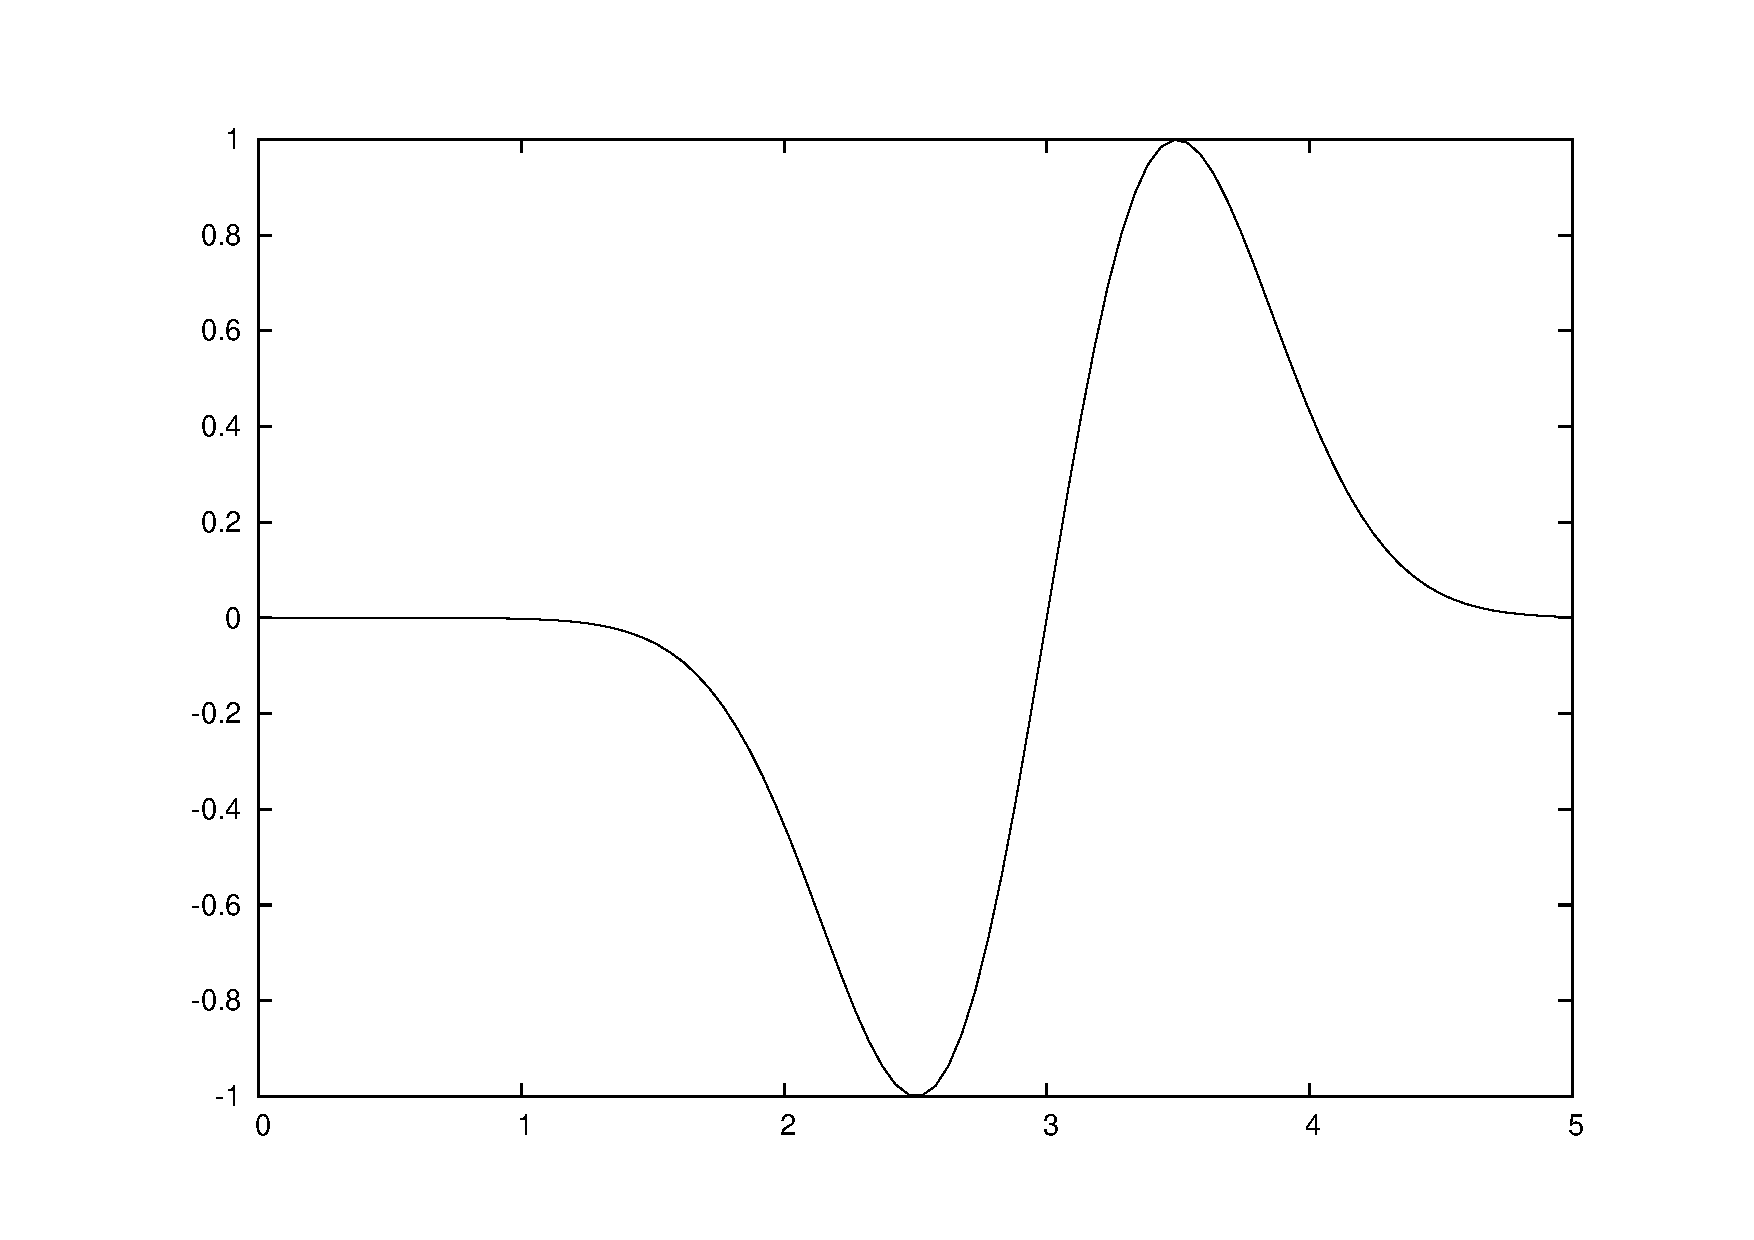
\includegraphics[width=14cm]{waveu}}
\caption{Input Displacement at Source Point ($\alpha=0.7$, $t_{0}=3$, $U_{0}=1$).}
\label{WAVE FIG 1.2}
\end{figure}

\begin{figure}
\centerline{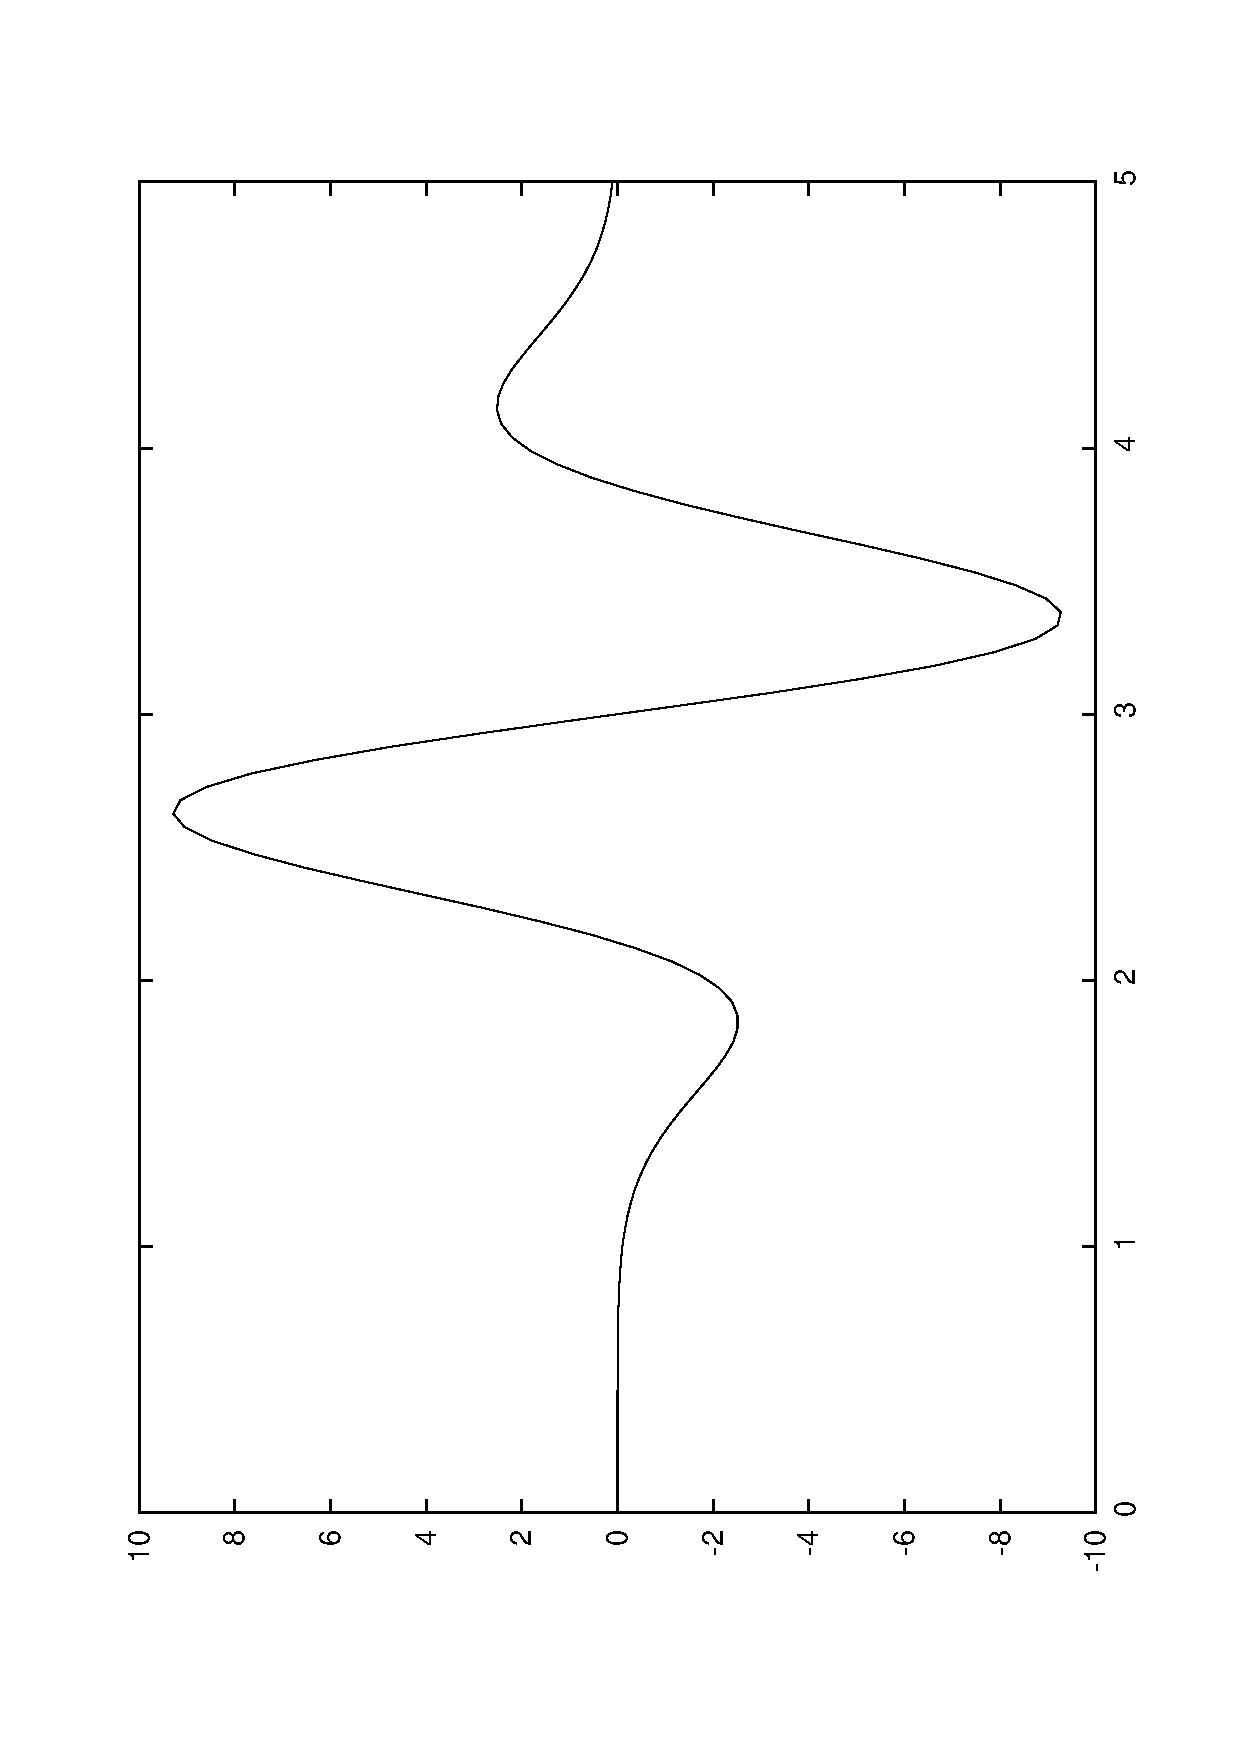
\includegraphics[width=14cm]{wavea}}
\caption{Input Acceleration at Source Point ($\alpha=0.7$, $t_{0}=3$, $U_{0}=1$).}
\label{WAVE FIG 1.1}
\end{figure}

Here we are modelling a point source at the point $x_C$ in the
$x_{0}$-direction which is a negative pulse of amplitude
$U_{0}$ followed by the same positive pulse.
In mathematical terms we use
\begin{eqnarray} \label{WAVE source}
u_{0}(x_C,t)= U_{0} \; \sqrt{2}  \frac{(t-t_{0})}{\alpha} e^{\frac{1}{2}-\frac{(t-t_{0})^2}{\alpha^2}} \ 
\end{eqnarray}
for all $t\ge0$ where $\alpha$ is the width of the pulse and $t_{0}$
is the time when the pulse changes from negative to positive.
In the simulations we will choose $\alpha=0.3$ and $t_{0}=2$ (see
\fig{WAVE FIG 1.2}) and apply the source as a constraint in a sphere of small
radius around the point $x_C$.  

We use an explicit time integration scheme to calculate the displacement field
$u$ at certain time marks $t^{(n)}$, where $t^{(n)}=t^{(n-1)}+h$ with time
step size $h>0$.
In the following the upper index ${(n)}$ refers to values at time $t^{(n)}$.
We use the Verlet scheme\index{Verlet scheme} with constant time step size $h$
which is defined by
\begin{eqnarray} \label{WAVE dyn 2}
u^{(n)}=2u^{(n-1)}-u^{(n-2)} + h^2 a^{(n)} \\
\end{eqnarray}
for all $n=2,3,\ldots$. It is designed to solve a system of equations of the form
\begin{eqnarray} \label{WAVE dyn 2b} 
u_{,tt}=G(u)
\end{eqnarray}
where one sets $a^{(n)}=G(u^{(n-1)})$.

In our case $a^{(n)}$ is given by
\begin{eqnarray}\label{WAVE dyn 3}
\rho a^{(n)}_{i}=\sigma^{(n-1)}_{ij,j}
\end{eqnarray}
and boundary conditions
\begin{eqnarray} \label{WAVE natural at n}
\sigma^{(n-1)}_{ij}n_{j}=0
\end{eqnarray}
derived from \eqn{WAVE natural} where 
\begin{eqnarray} \label{WAVE dyn 3a}
\sigma_{ij}^{(n-1)} & = & \lambda u^{(n-1)}_{k,k} \delta_{ij} + \mu ( u^{(n-1)}_{i,j} + u^{(n-1)}_{j,i}).
\end{eqnarray}
We also need to apply the constraint 
\begin{eqnarray} \label{WAVE dyn 3aa}
a^{(n)}_{0}(x_C,t)= U_{0} 
\frac{\sqrt(2.)}{\alpha^2} (4\frac{(t-t_{0})^3}{\alpha^3}-6\frac{t-t_{0}}{\alpha})e^{\frac{1}{2}-\frac{(t-t_{0})^2}{\alpha^2}}
\end{eqnarray}
which is derived from equation~\ref{WAVE source} by calculating the second
order time derivative (see \fig{WAVE FIG 1.1}).
Now we have converted our problem for displacement, $u^{(n)}$, into a problem
for acceleration, $a^{(n)}$, which depends on the solution at the previous two
time steps $u^{(n-1)}$ and $u^{(n-2)}$.

In each time step we have to solve this problem to get the acceleration $a^{(n)}$,
and we will use the \LinearPDE class of the \linearPDEs package to do so.
The general form of the PDE defined through the \LinearPDE class is discussed
in \Sec{SEC LinearPDE}. The form which is relevant here is
\begin{equation}\label{WAVE dyn 100}
D_{ij} a^{(n)}_{j} = - X_{ij,j}\; .
\end{equation}
The natural boundary condition
\begin{equation}\label{WAVE dyn 101}
n_{j}X_{ij} =0 
\end{equation}
is used. 
With $u=a^{(n)}$ we can identify the values to be assigned to $D$ and $X$:
\begin{equation}\label{WAVE dyn 6}
\begin{array}{ll}
D_{ij}=\rho \delta_{ij}&
X_{ij}=-\sigma^{(n-1)}_{ij}\\
\end{array}
\end{equation}
Moreover we need to define the location $r$ where the constraint~\ref{WAVE dyn 3aa} is applied.
We will apply the constraint on a small sphere of radius $R$ around
$x_C$ (we will use 3\% of the width of the domain):  
\begin{equation}\label{WAVE dyn 6 1}
q_{i}(x) = 
\left\{
\begin{array}{l l}
    1 & \quad \text{where $\|x-x_c\|\le R$}\\
    0 & \quad \text{otherwise}
\end{array}
\right.
\end{equation}
The following script defines the function \function{wavePropagation} which
implements the Verlet scheme to solve our wave propagation problem.
The argument \var{domain} which is a \Domain class object defines the domain
of the problem.
\var{h} and \var{tend} are the time step size and the end time of the simulation.
\var{lam}, \var{mu} and \var{rho} are material properties.
\begin{python}
  def wavePropagation(domain,h,tend,lam,mu,rho, x_c, src_radius, U0):
     # lists to collect displacement at point source which is returned
     # to the caller
     ts, u_pc0, u_pc1, u_pc2 = [], [], [], []
    
     x=domain.getX()
     # ... open new PDE ...
     mypde=LinearPDE(domain)
     mypde.getSolverOptions().setSolverMethod(mypde.getSolverOptions().HRZ_LUMPING)
     kronecker=identity(mypde.getDim())
     dunit=numpy.array([1., 0., 0.]) # defines direction of point source
     mypde.setValue(D=kronecker*rho, q=whereNegative(length(x-xc)-src_radius)*dunit)
     # ... set initial values ....
     n=0
     # for first two time steps
     u=Vector(0., Solution(domain))
     u_last=Vector(0., Solution(domain))
     t=0
     # define the location of the point source 
     L=Locator(domain, xc)
     # find potential at point source
     u_pc=L.getValue(u)
     print("u at point charge=",u_pc)
     ts.append(t)
     u_pc0.append(u_pc[0])
     u_pc1.append(u_pc[1])
     u_pc2.append(u_pc[2])
  
     while t<tend:
       t+=h
       # ... get current stress ....
       g=grad(u)
       stress=lam*trace(g)*kronecker+mu*(g+transpose(g))
       # ... get new acceleration ....
       amplitude=U0*(4*(t-t0)**3/alpha**3-6*(t-t0)/alpha)*sqrt(2.)/alpha**2 \
                                               *exp(1./2.-(t-t0)**2/alpha**2)
       mypde.setValue(X=-stress, r=dunit*amplitude)
       a=mypde.getSolution()
       # ... get new displacement ...
       u_new=2*u-u_last+h**2*a
       # ... shift displacements ....
       u_last=u
       u=u_new
       n+=1
       print(n,"-th time step, t=",t)
       u_pc=L.getValue(u)
       print("u at point charge=",u_pc)
       # save displacements at point source to file for t > 0
       ts.append(t)
       u_pc0.append(u_pc[0])
       u_pc1.append(u_pc[1])
       u_pc2.append(u_pc[2])
  
       # ... save current acceleration in units of gravity and displacements 
       if n==1 or n%10==0:
         saveVTK("./data/usoln.%i.vtu"%(n/10), \
                 acceleration = length(a)/9.81, \
                 displacement = length(u), \
  				 tensor = stress, Ux = u[0])
  
     return ts, u_pc0, u_pc1, u_pc2
\end{python}
Notice that all coefficients of the PDE which are independent of time $t$ are
set outside the \code{while} loop.
This is for efficiency reasons since it allows the \LinearPDE class to reuse
information as much as possible when iterating over time. 

The statement
\begin{python}
  mypde.getSolverOptions().setSolverMethod(mypde.getSolverOptions().HRZ_LUMPING) 
\end{python}
switches on the use of an aggressive approximation of the PDE operator as a
diagonal matrix formed from the coefficient \var{D}.
The approximation allows, at the cost of additional error, very fast solution
of the PDE, see also Section~\ref{REMARKS ON LUMPING}.

There are a few new \escript functions in this example: 
\code{grad(u)} returns the gradient $u_{i,j}$ of $u$ (in fact \var{grad(g)[i,j]}$==u_{i,j}$).
There are restrictions on the argument of the \function{grad} function, for
instance the statement \code{grad(grad(u))} will raise an exception.
\code{trace(g)} returns the sum of the main diagonal elements \var{g[k,k]} of
\var{g} and \code{transpose(g)} returns the matrix transpose of \var{g} (i.e.
$\var{transpose(g)[i,j]}==\var{g[j,i]}$). 

We initialize the values of \code{u} and \code{u_last} to be zero.
It is important to initialize both with the \SolutionFS as they have to be
seen as solutions of PDEs from previous time steps.
In fact, the \function{grad} does not accept arguments with a certain
\FunctionSpace, for more details see \Sec{SEC ESCRIPT DATA}. 

The \class{Locator} class is designed to extract values at a given location
(in this case $x_C$) from functions such as the displacement vector \code{u}.
Typically \class{Locator} is used in the following way:
\begin{python}
  L=Locator(domain, xc)
  u=...
  u_pc=L.getValue(u)
\end{python}
The return value \code{u_pc} is the value of \code{u} at the location
\code{xc}\footnote{In fact, it is the finite element node which is closest to
the given position. The usage of \class{Locator} is MPI safe.}.
The values are collected in the lists \var{u_pc0}, \var{u_pc1} and \var{u_pc2}
together with the corresponding time marker in \var{ts}.
These values are handed back to the caller. Later we will show ways to access these data.

One of the big advantages of the Verlet scheme is the fact that the problem to
be solved in each time step is very simple and does not involve any spatial
derivatives (which is what allows us to use lumping in this simulation).
The problem becomes so simple because we use the stress from the last time
step rather than the stress which is actually present at the current time step.
Schemes using this approach are called explicit time integration schemes\index{explicit scheme}\index{time integration!explicit}.
The backward Euler scheme we have used in \Chap{DIFFUSION CHAP} is an example
of an implicit scheme\index{implicit scheme}\index{time integration!implicit}.
In this case one uses the actual status of each variable at a particular time
rather than values from previous time steps.
This will lead to a problem which is more expensive to solve, in particular
for non-linear cases.
Although explicit time integration schemes are cheap to finalize a single time
step, they need significantly smaller time steps than implicit schemes and can
suffer from stability problems.
Therefore they require a very careful selection of the time step size $h$.

An easy, heuristic way of choosing an appropriate time step size is the
Courant–Friedrichs–Lewy condition (CFL condition)\index{Courant condition}\index{explicit scheme!Courant condition}
which says that within a time step information should not travel further than
a cell used in the discretization scheme.
In the case of the wave equation the velocity of a (p-) wave is given as
$\sqrt{\frac{\lambda+2\mu}{\rho}}$ so one should choose $h$ from
\begin{eqnarray}\label{WAVE dyn 66}
h= \frac{1}{5} \sqrt{\frac{\rho}{\lambda+2\mu}} \Delta x
\end{eqnarray}
where $\Delta x$ is the cell diameter.
The factor $\frac{1}{5}$ is a safety factor considering the heuristics of the formula. 

\begin{figure}[t]
\begin{center}
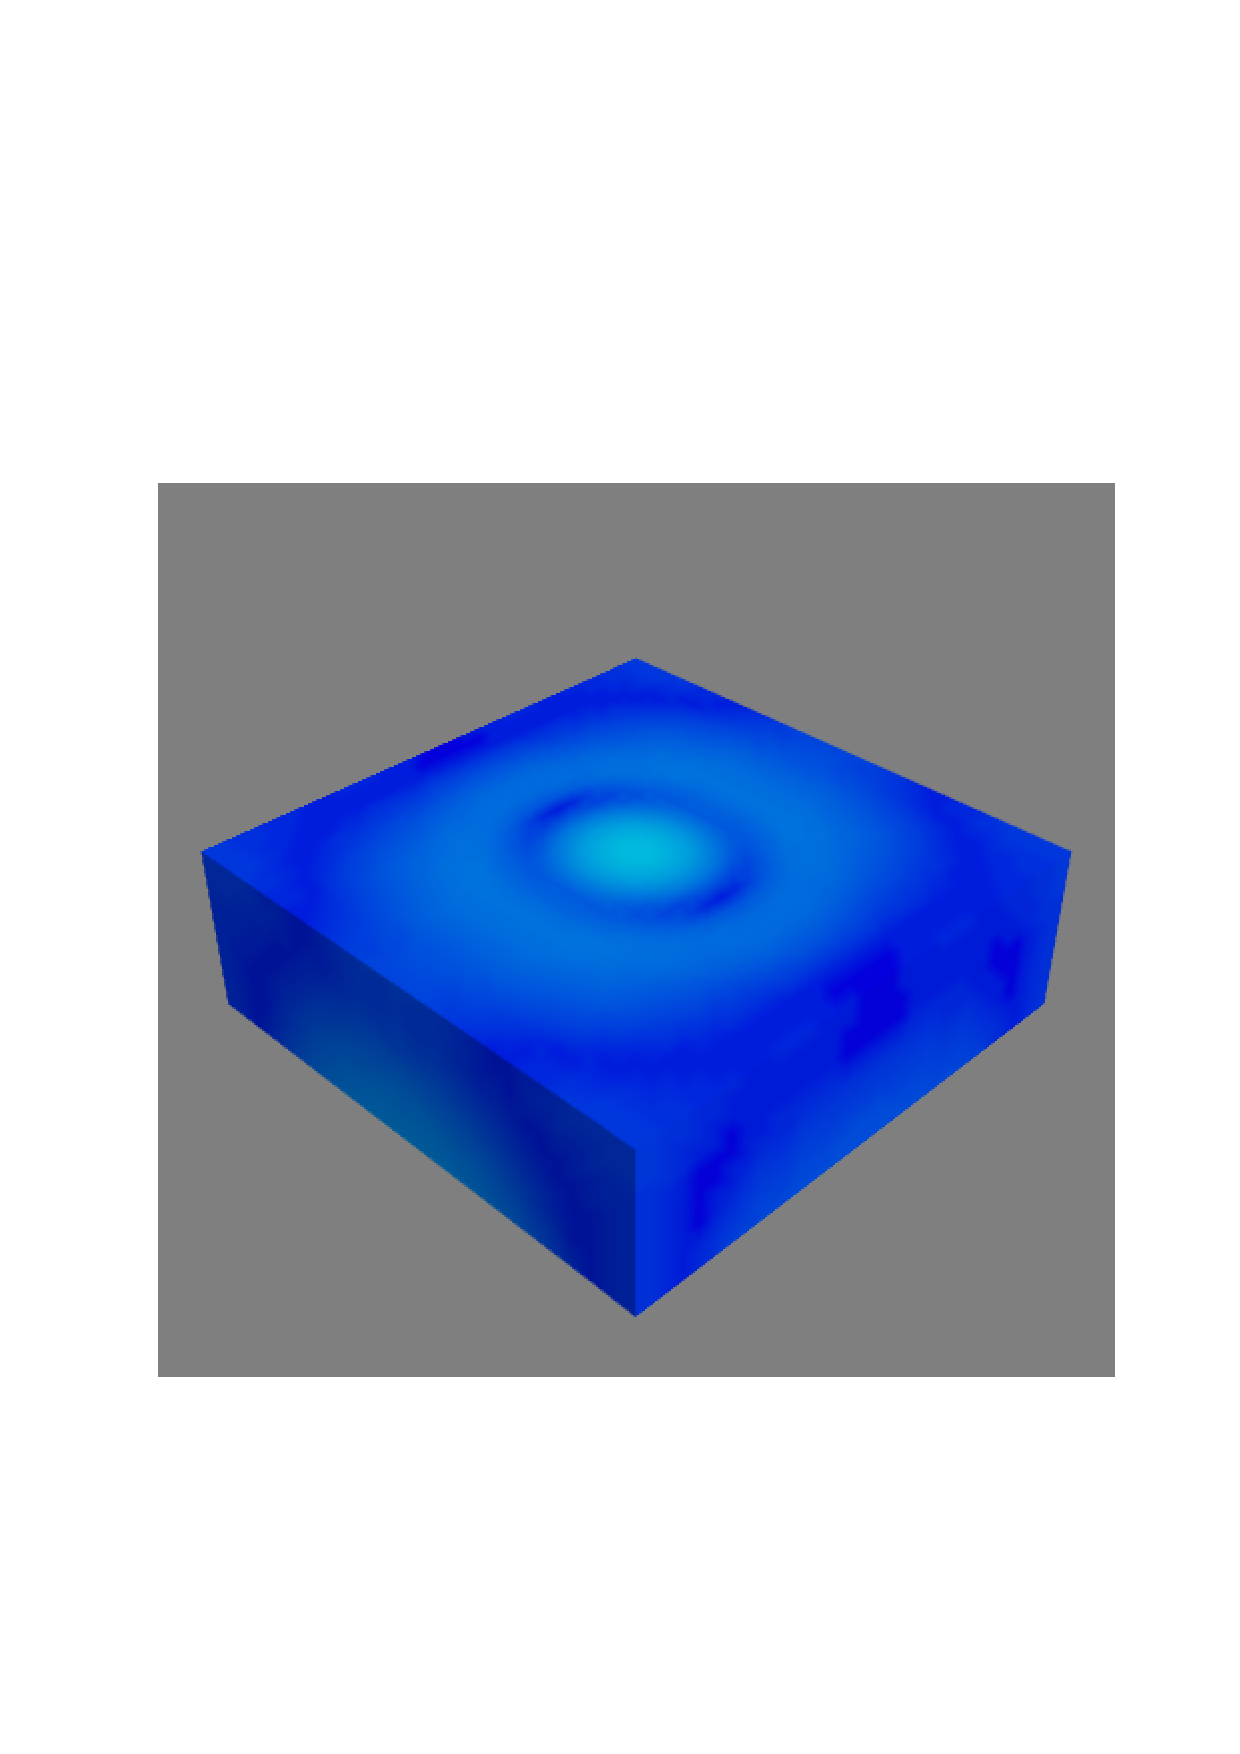
\includegraphics[width=2in]{Wave11}
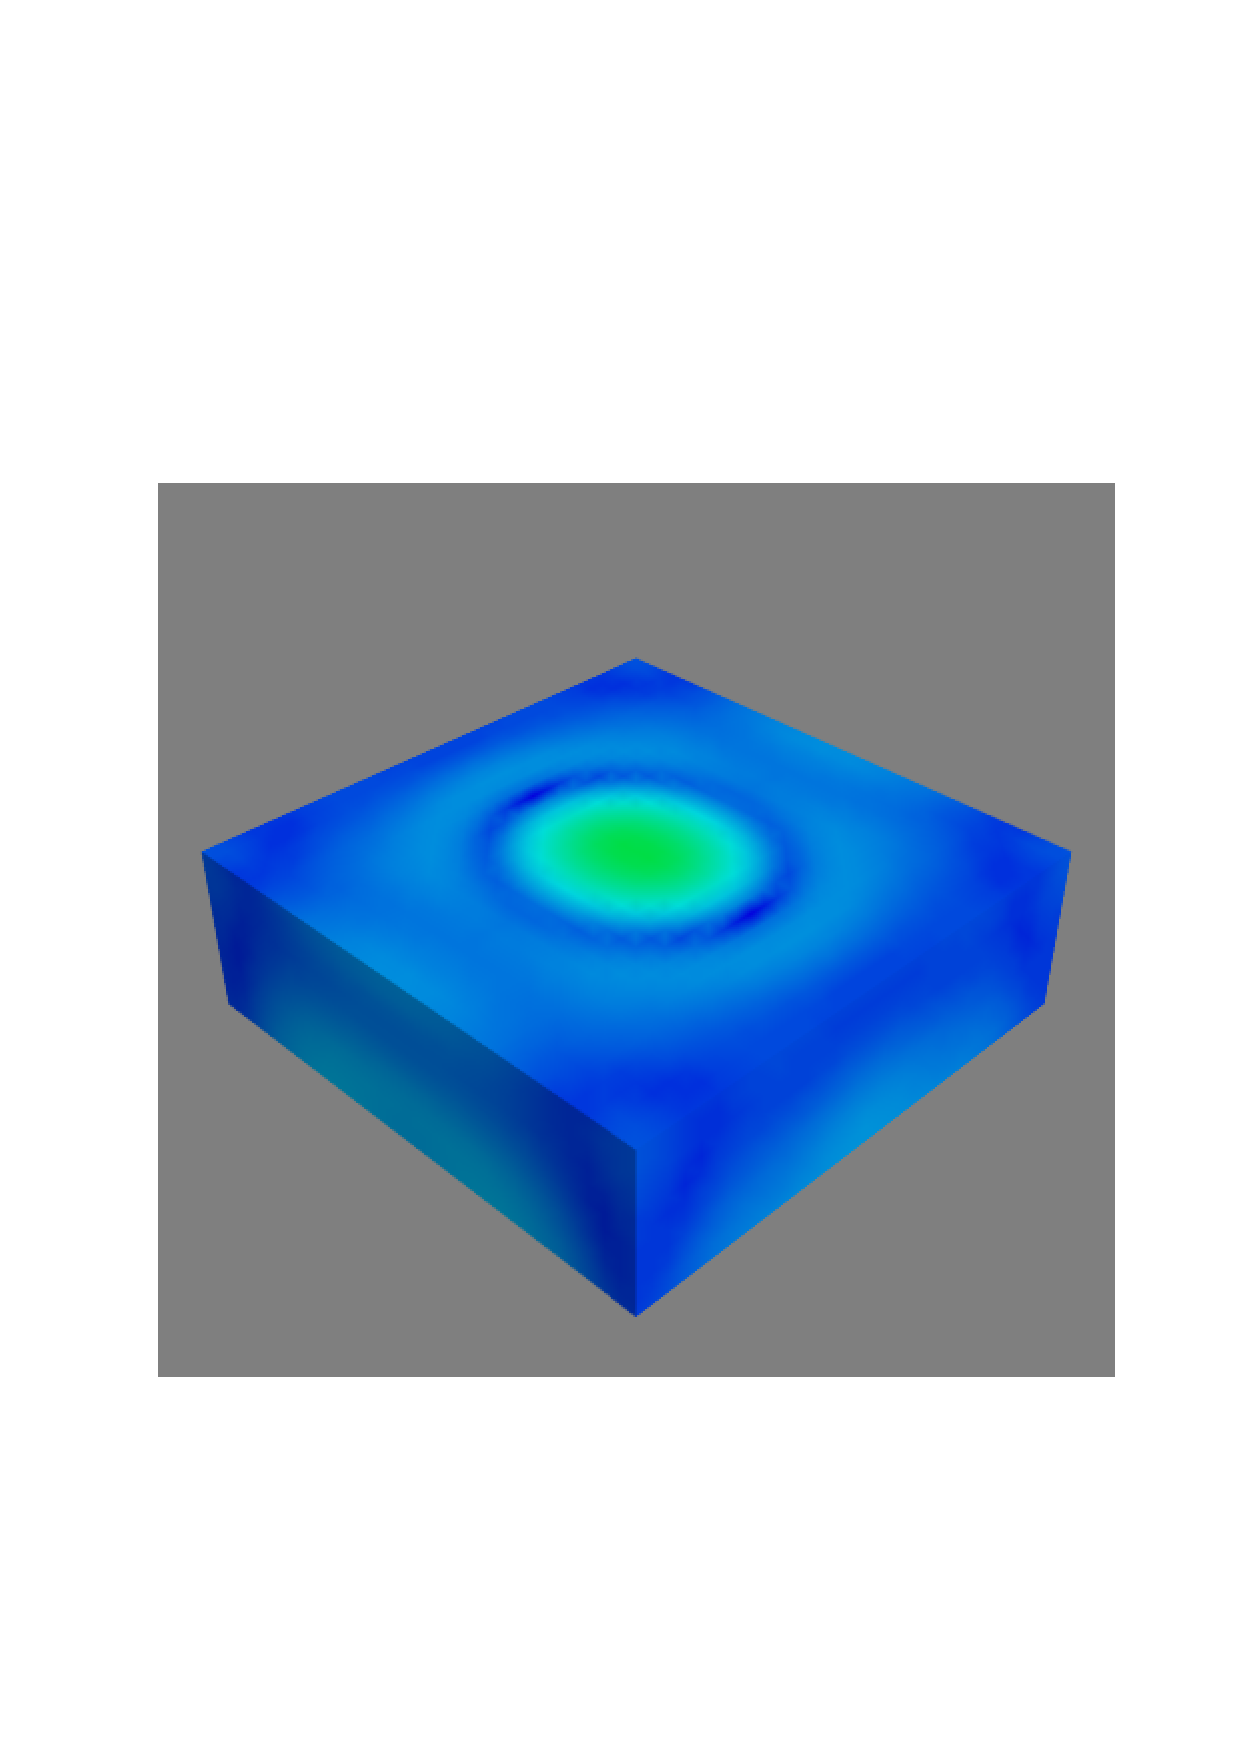
\includegraphics[width=2in]{Wave22}
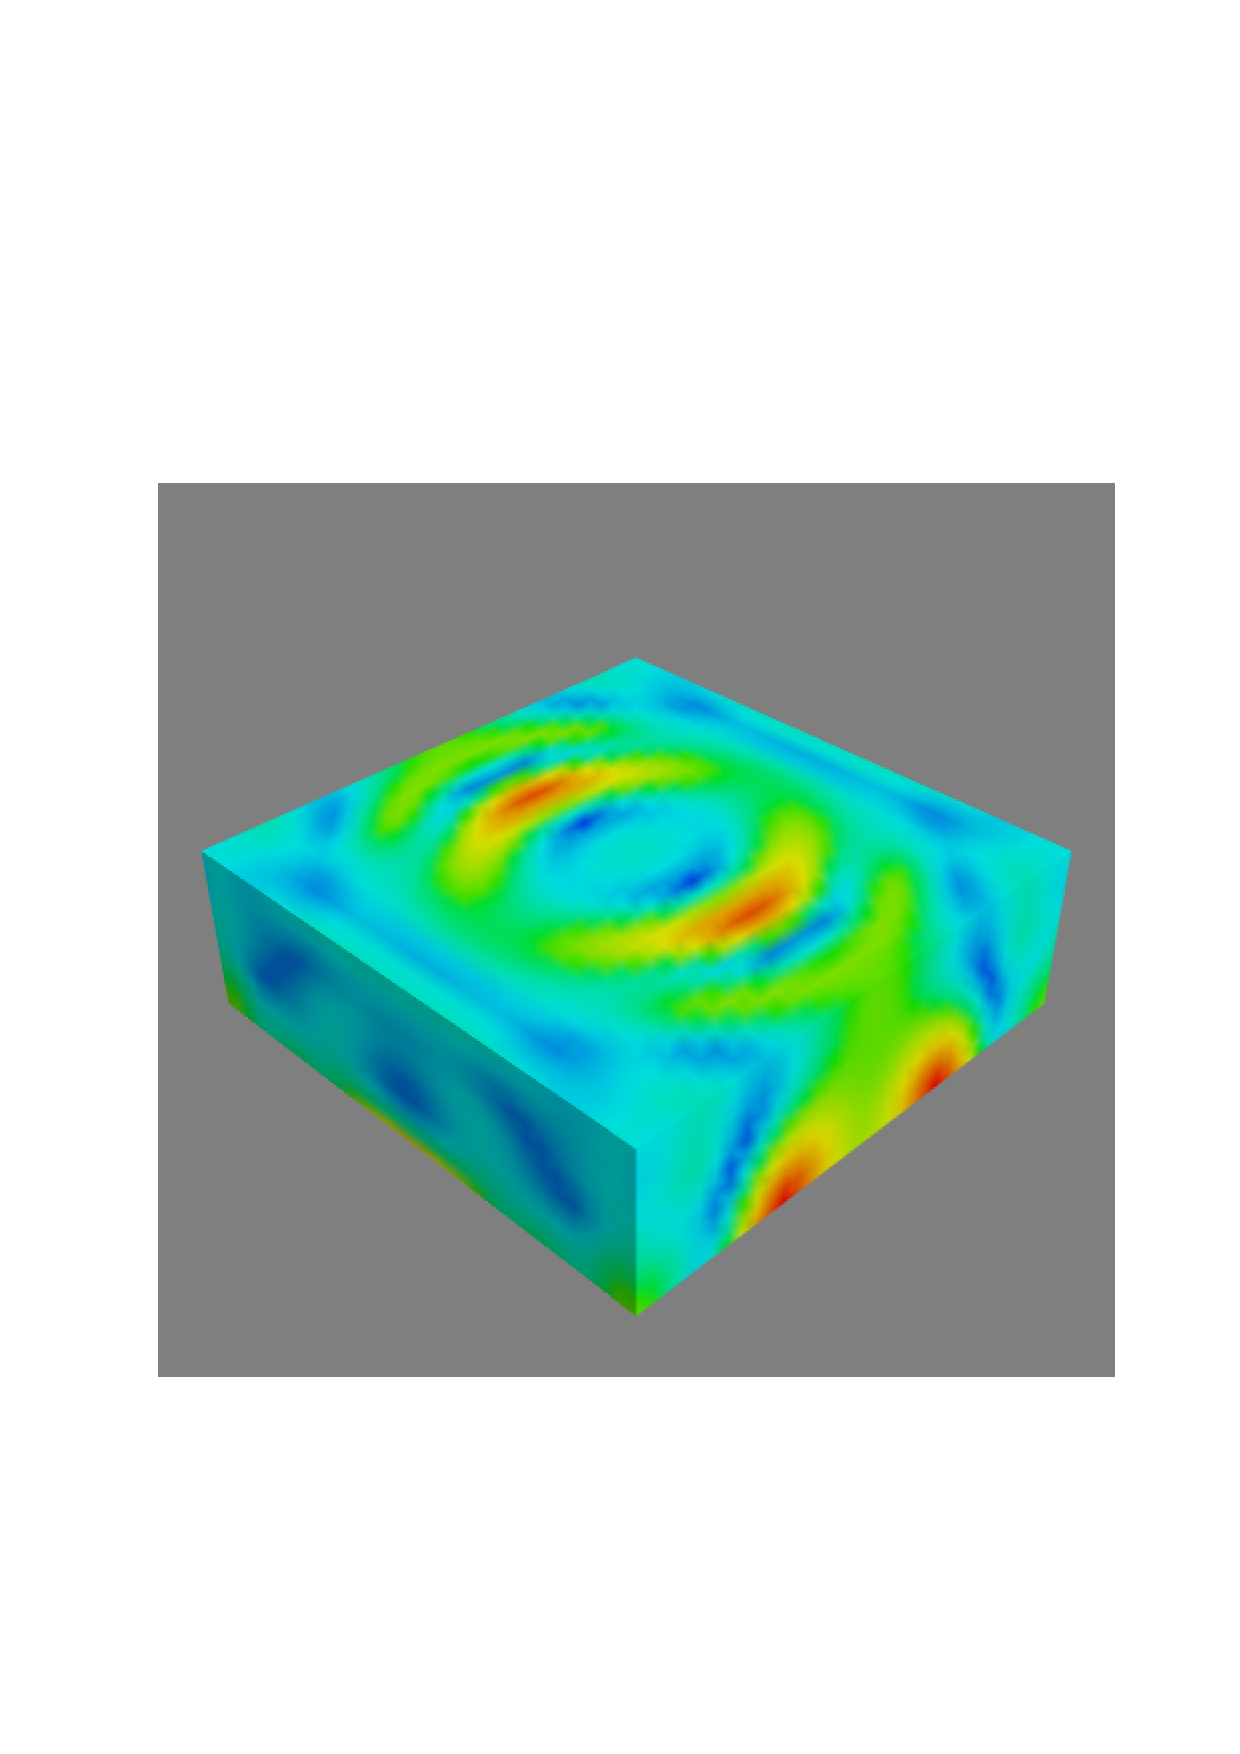
\includegraphics[width=2in]{Wave28}
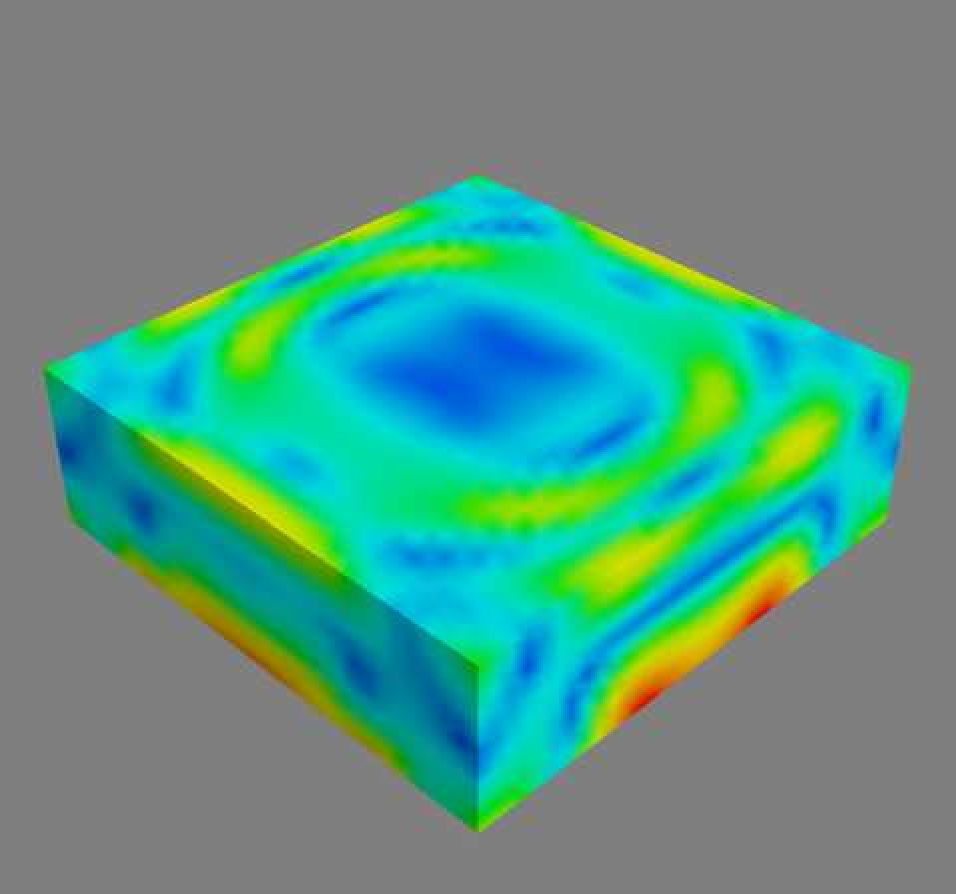
\includegraphics[width=2in]{Wave32}
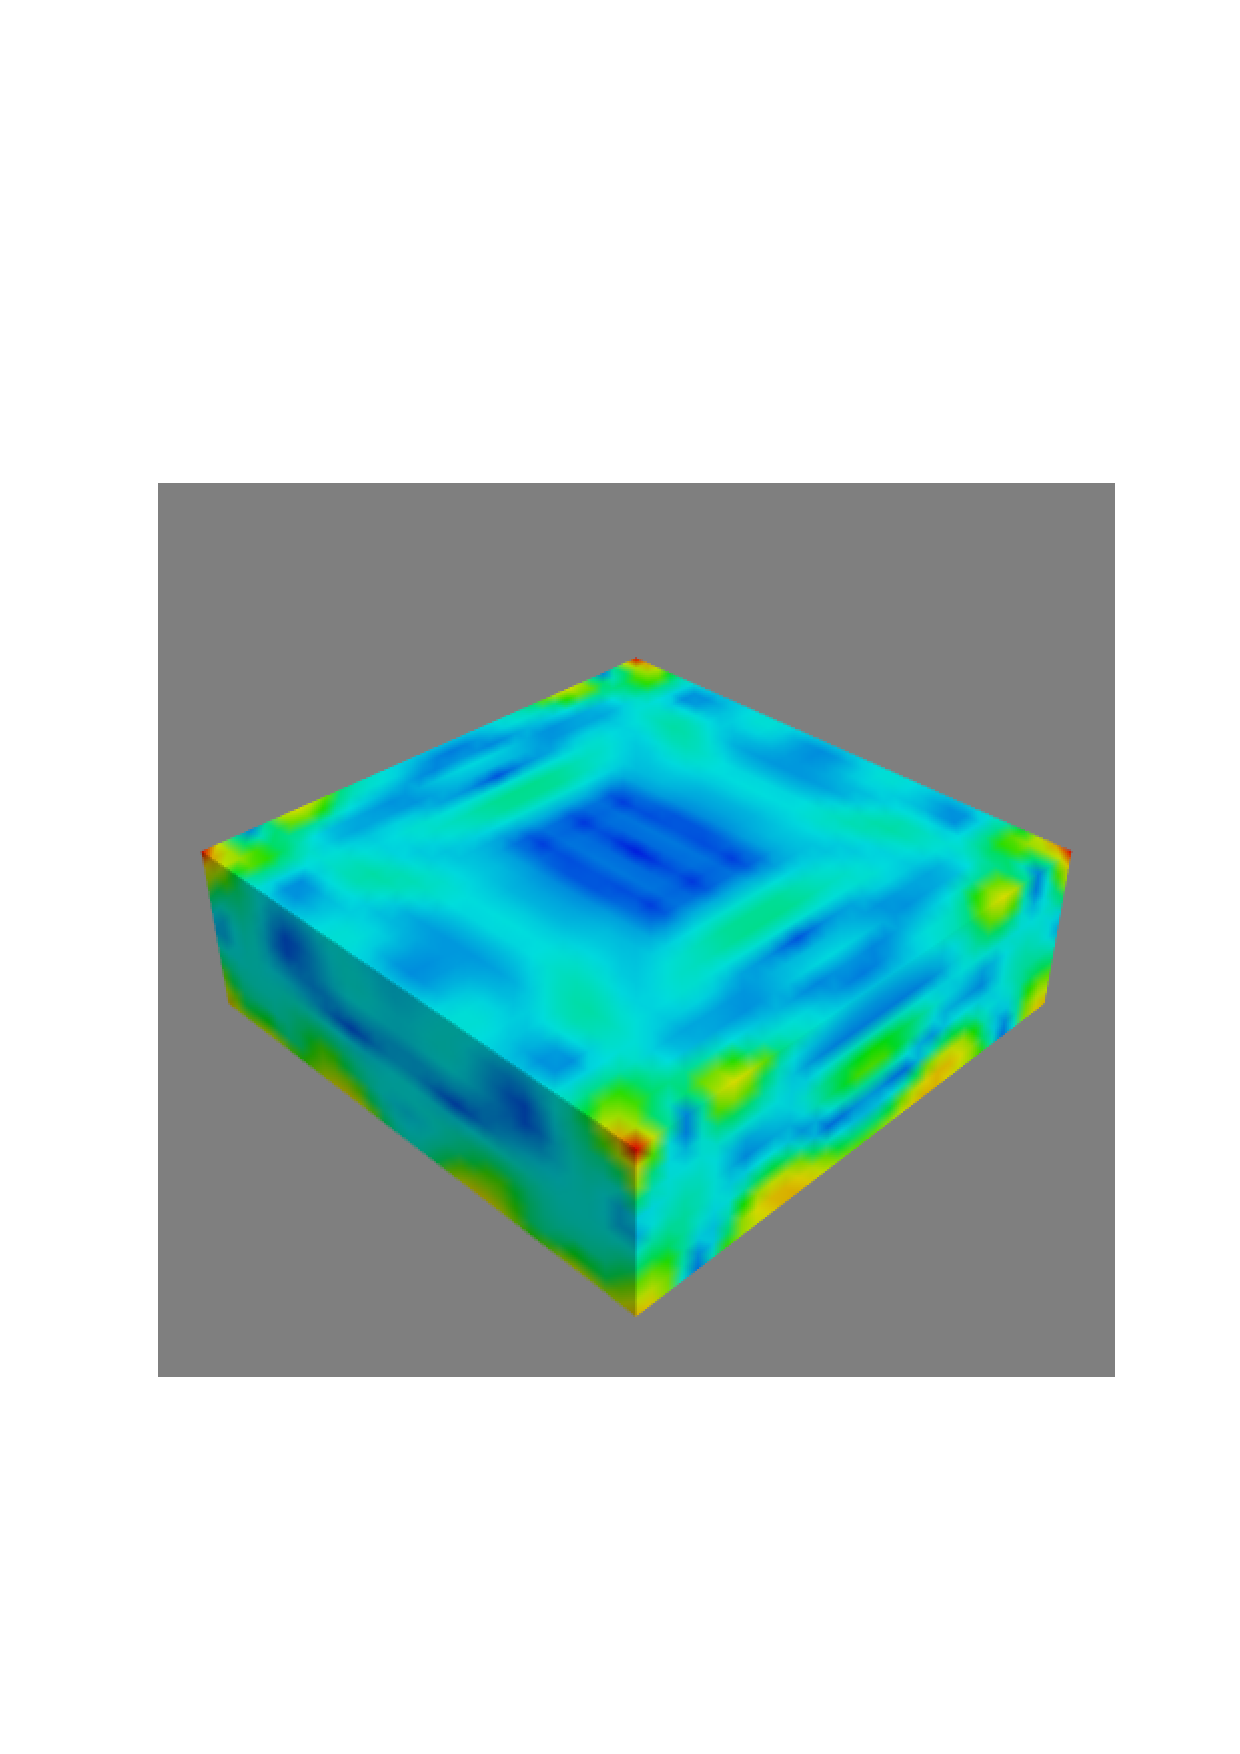
\includegraphics[width=2in]{Wave36}
\end{center}
\caption{Selected time steps ($n = 11, 22, 32, 36$) of a wave propagation over
a 10km $\times$ 10km $\times$ 3.125km block from a point source initially at
(5km, 5km, 0) with time step size $h=0.02083$. Color represents the
displacement. Here the view is oriented onto the bottom face.
\label{WAVE FIG 2}}
\end{figure}

The following script uses the \code{wavePropagation} function to solve the
wave equation for a point source located at the bottom face of a block.
The width of the block in each direction on the bottom face is 10km
($x_0$ and $x_1$ directions, i.e. \code{l0} and \code{l1}).
The variable \code{ne} gives the number of elements in $x_{0}$ and $x_1$ directions.
The depth of the block is aligned with the $x_{2}$-direction.
The depth (\code{l2}) of the block in the $x_{2}$-direction is chosen
so that there are 10 elements, and the magnitude of the depth is chosen such
that the elements become cubic.
We chose 10 for the number of elements in the $x_{2}$-direction so
that the computation is faster. \code{Brick($n_0,  n_1, n_2,l_0,l_1,l_2$)}
is an \finley function which creates a rectangular mesh with $n_0 \times n_1 \times n_2$
elements over the brick $[0,l_0] \times [0,l_1] \times [0,l_2]$.
\begin{python}
  from esys.finley import Brick
  ne = 32          # number of cells in x_0 and x_1 directions
  width = 10000.   # length in x_0 and x_1 directions
  lam = 3.462e9
  mu = 3.462e9
  rho = 1154.
  tend = 60
  U0 = 1. # amplitude of point source
  # spherical source at middle of bottom face
  xc=[width/2.,width/2.,0.]
  # define small radius around point xc
  src_radius = 0.03*width
  print("src_radius =",src_radius)
  mydomain=Brick(ne, ne, 10, l0=width, l1=width, l2=10.*width/32.)
  h=(1./5.)*inf(sqrt(rho/(lam+2*mu))*inf(domain.getSize())
  print("time step size =",h)
  ts, u_pc0, u_pc1, u_pc2 =  \
          wavePropagation(mydomain, h, tend, lam, mu, rho, xc, src_radius, U0)
\end{python}
The \function{domain.getSize()} function returns the local element size $\Delta x$.
Using \function{inf} ensures that the CFL condition~\ref{WAVE dyn 66} \index{Courant number}\index{CFL condition} holds
everywhere in the domain. 

The script is available as \file{wave.py} in the \ExampleDirectory\index{scripts!\file{wave.py}}. 
To visualize the results from the data directory:
\begin{verbatim} 
mayavi2 -d usoln.1.vtu -m SurfaceMap
\end{verbatim}
You can rotate this figure by clicking on it with the mouse and moving it around.
Again use \emph{Configure Data} to move backward and forward in time, and
also to choose the results (acceleration, displacement or $u_x$) by
using \emph{Select Scalar}.
\fig{WAVE FIG 2} shows the results for the displacement at various time steps.

\begin{figure}[t!]
\centerline{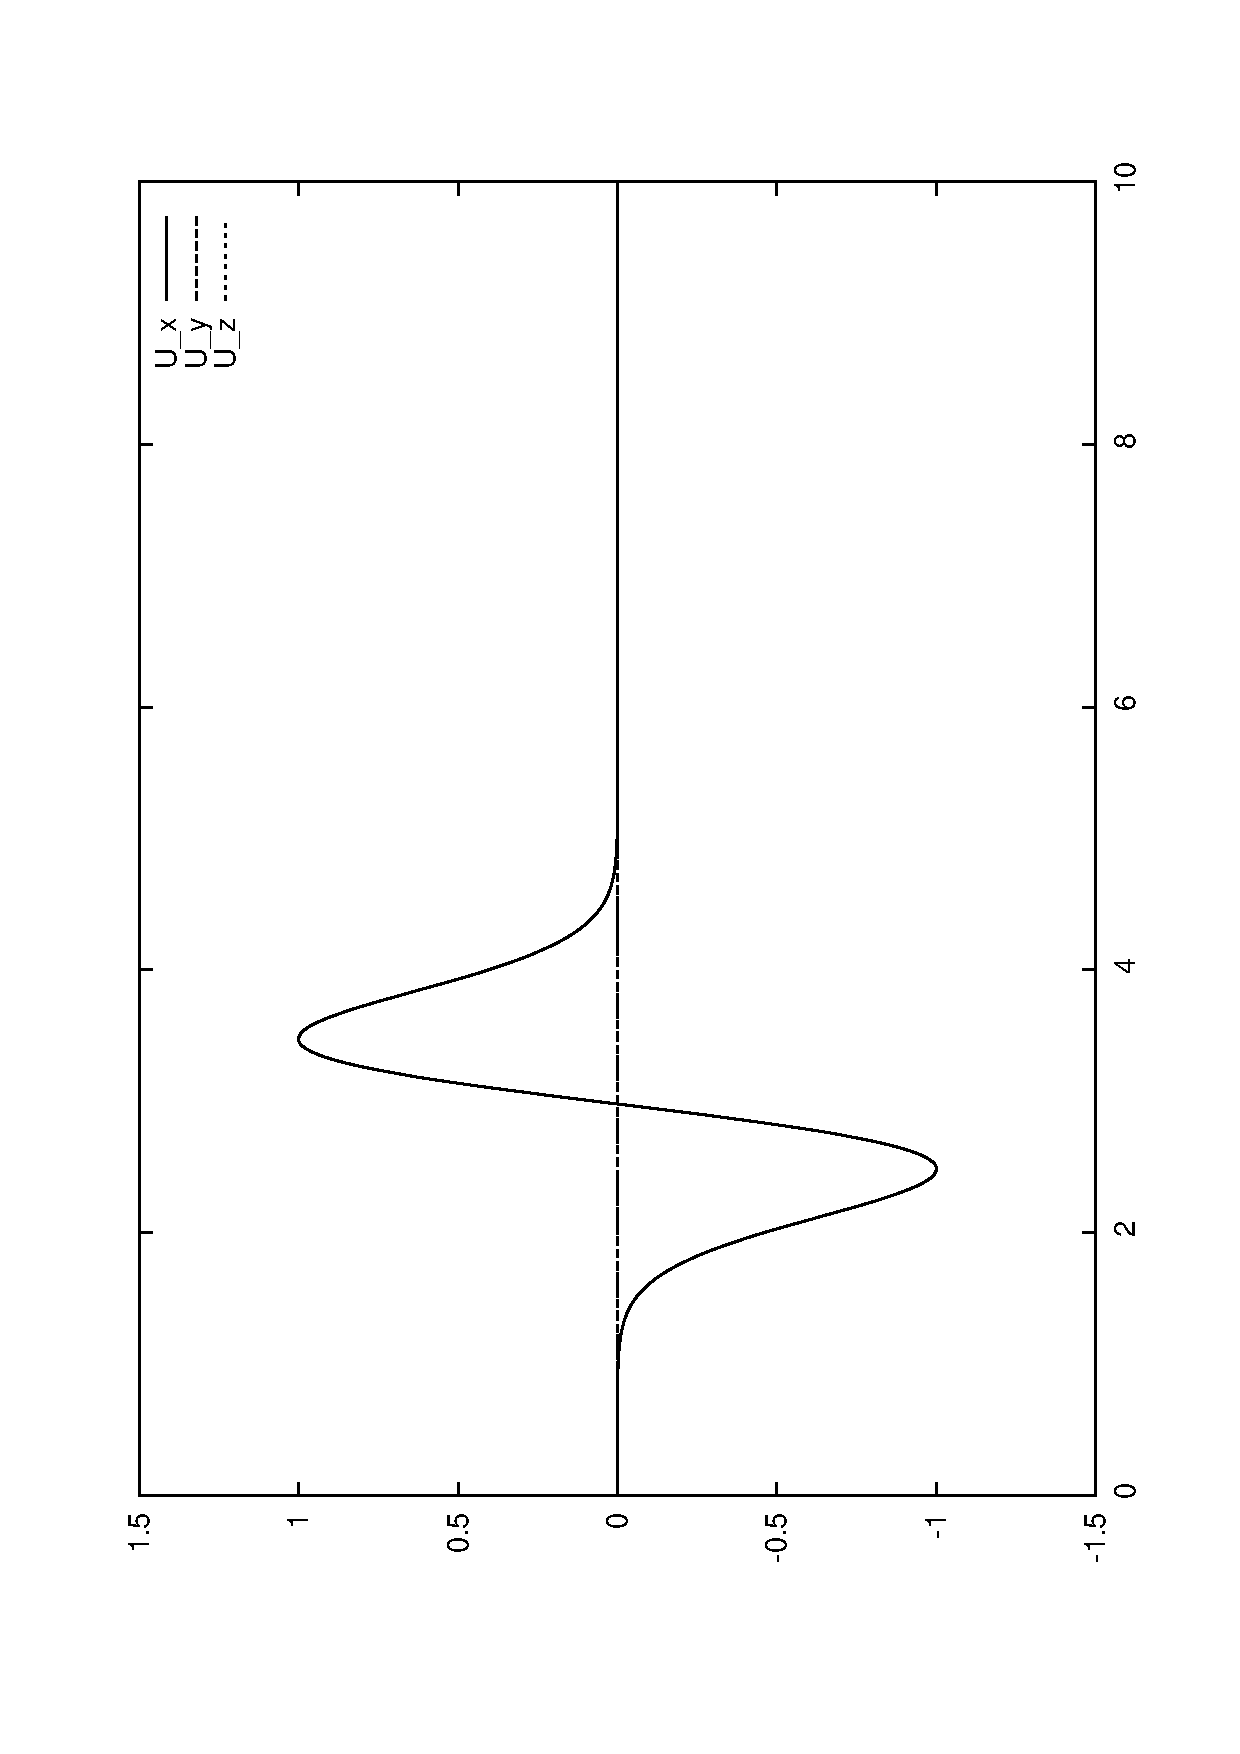
\includegraphics[width=14cm]{WavePC}}
\caption{Amplitude at Point source from the Simulation}
\label{WAVE FIG 1}
\end{figure}

It remains to show some possibilities to inspect the collected data
\var{u_pc0}, \var{u_pc1} and \var{u_pc2}.
One way is to write the data to a file and then use an external package such
as \gnuplot, Excel or OpenOffice.org Calc to read the data for further analysis.
The following code shows one possible way to write the data to the file \file{./data/U_pc.csv}:
\begin{python}
  u_pc_data=FileWriter('./data/U_pc.csv')
  for i in xrange(len(ts)):
      u_pc_data.write("%f %f %f %f\n"%(ts[i],u_pc0[i],u_pc1[i],u_pc2[i]))
  u_pc_data.close()
\end{python}
The file \code{U_pc.csv} stores 4 columns of data: $t,u_x,u_y,u_z$
respectively, where $u_x,u_y,u_z$ are the
$x_0,x_1,x_2$ components of the displacement
vector $u$ at the point source.
These can be plotted easily using any plotting package.
In \gnuplot the command:
\begin{verbatim}
 plot 'U_pc.csv' u 1:2 title 'U_x' w l lw 2, 'U_pc.csv' u 1:3 title 'U_y' w l
lw 2, 'U_pc.csv' u 1:4 title 'U_z' w l lw 2
\end{verbatim}
will reproduce \fig{WAVE FIG 1} (As expected this is identical to the input
signal shown in \fig{WAVE FIG 1.2}).
It is pointed out that we are not using the standard \PYTHON \function{open}
to write to the file \code{U_pc.csv} as it is not safe when running \escript
under MPI, see Chapter~\ref{EXECUTION} for more details.

Alternatively, one can implement plotting the results at run time rather than
in a post-processing step.
This avoids the generation of an intermediate data file.
In {\it escript} the preferred way of creating 2D plots of time dependent data
is \MATPLOTLIB. The following script creates the plot and writes it into the
file \file{u_pc.png} in the PNG image format:
\begin{python}
  import matplotlib.pyplot as plt
  if getMPIRankWorld() == 0:
      plt.title("Displacement at Point Source")
      plt.plot(ts, u_pc0, '-', label="x_0", linewidth=1)
      plt.plot(ts, u_pc1, '-', label="x_1", linewidth=1)
      plt.plot(ts, u_pc2, '-', label="x_2", linewidth=1)
      plt.xlabel('time')
      plt.ylabel('displacement')
      plt.legend()
      plt.savefig('u_pc.png', format='png')
\end{python}
You can add \function{plt.show()} to create an interactive browser window.
Notice that by checking the condition \code{getMPIRankWorld()==0} the plot
is generated on one processor only (in this case the rank 0 processor) when
run under \MPI. 

Both options for processing the point source data are include in the example
file \file{wave.py}. There are other options available to process these data
in particular through the \SCIPY package, e.g. Fourier transformations.
It is beyond the scope of this user's guide to document the usage of
\SCIPY for time series analysis but it is highly recommended that users use
\SCIPY for any further data processing.

